\documentclass[15pt]{sprawozdanie}
\usepackage{soul}

% \class{Praca dyplomowa inżynierska}
% \title{Opracowanie wirtualnego środowiska do symulacji dynamiki lotu bezzałogowych statków powietrznych}
\class{Seminarium dyplomowe -- prezetacja I, konspekt}
\title{Wirtualne środowisko do symulacji dynamiki lotu bezzałogowych statków powietrznych}
\author{\textbf{inż. Wojciech Gajda} 304494\\\vspace{20pt}\textbf{Igor Faliszewski} 313223}
\instructor{dr inż. Paweł Kotowski}
\deadline{\today}

\graphicspath{{images/}}

\usepackage{amssymb}
\usepackage{amsmath}
\usepackage{polski}
\usepackage[utf8]{inputenc}
\usepackage{hyperref}
\usepackage{blindtext}
\usepackage{multicol}
\usepackage{multirow}
\usepackage{wrapfig}
\usepackage{float}
\usepackage{enumitem}
\usepackage{xfrac}
\usepackage{caption}
\usepackage{subcaption}
\usepackage{booktabs}
\usepackage{wasysym}
\usepackage{xcolor}
\usepackage{listings}
\usepackage{pdfpages}
\usepackage{fontspec}
\usepackage{comment}

\setmainfont{Verdana}
	
\usepackage{color, colortbl}
\definecolor{Gray}{gray}{0.9}

\definecolor{mGreen}{rgb}{0,0.6,0}
\definecolor{mGray}{rgb}{0.5,0.5,0.5}
\definecolor{mPurple}{rgb}{0.58,0,0.82}
\definecolor{backgroundColour}{rgb}{0.95,0.95,0.92}

\lstdefinestyle{CStyle}{
    backgroundcolor=\color{backgroundColour},   
    commentstyle=\color{mGreen},
    keywordstyle=\color{magenta},
    numberstyle=\tiny\color{mGray},
    stringstyle=\color{mPurple},
    basicstyle=\footnotesize,
    breakatwhitespace=false,         
    breaklines=true,                 
    captionpos=b,                    
    keepspaces=true,                 
    numbers=left,                    
    numbersep=5pt,                  
    showspaces=false,                
    showstringspaces=false,
    showtabs=false,                  
    tabsize=2,
    language=C
}

\usepackage[
backend=biber
,style=ieee
,sorting=none
]{biblatex}
\addbibresource{bibliografia.bib}
\DeclareNameAlias{author}{last-first}

\DeclareCiteCommand{\supercite}[\mkbibsuperscript]
  {\iffieldundef{prenote}
     {}
     {\BibliographyWarning{Ignoring prenote argument}}%
   \iffieldundef{postnote}
     {}
     {\BibliographyWarning{Ignoring postnote argument}}}
  {\usebibmacro{citeindex}%
   \bibopenbracket\usebibmacro{cite}\bibclosebracket}
  {\supercitedelim}
  {}
  
  \DeclareLabelalphaTemplate{
  \labelelement{
    \field[final]{shorthand}
    \field{label}
    \field[strwidth=3,strside=left,ifnames=1]{labelname}
    \field[strwidth=1,strside=left,final]{labelname}
    \field{labeltitle}
  }
  \labelelement{
    \field[strwidth=2,strside=right]{year}
  }
}

%\let\cite=\supercite

\renewcommand*{\figurename}{Rys.}

\usepackage{titlesec}
\titlelabel{\thetitle.\quad}

\usepackage{tikz}


\usetikzlibrary{matrix, ,backgrounds}
\usepackage{array}

\makeatletter
\tikzset{SWOT/.style={matrix of nodes,inner sep=0pt,row sep=0pt,column sep=0pt,
cells={nodes={anchor=center,inner sep=2pt}},
column 1/.style={nodes={rotate=90,minimum height=8mm}},
ampersand replacement=\&,
execute at end matrix={\begin{scope}[on background layer]
 \fill[black!10] (\tikz@fig@name.west|-\tikz@fig@name-2-2.north) rectangle 
  (\tikz@fig@name-\the\pgfmatrixcurrentrow-2.south west);
\end{scope}
\draw (\tikz@fig@name.west|-\tikz@fig@name-2-2.north) rectangle 
(\tikz@fig@name-\the\pgfmatrixcurrentrow-\the\pgfmatrixcurrentcolumn.south east)
 (\tikz@fig@name-1-2.north west) rectangle 
(\tikz@fig@name-\the\pgfmatrixcurrentrow-\the\pgfmatrixcurrentcolumn.south east)
(\tikz@fig@name-2-2.center|-\tikz@fig@name.north) --
 (\tikz@fig@name-2-2.center|-\tikz@fig@name.south)
foreach \XX in {2,...,\the\numexpr\pgfmatrixcurrentrow-1}
{(\tikz@fig@name-\XX-2.south-|\tikz@fig@name.west) --
(\tikz@fig@name-\XX-2.south-|\tikz@fig@name.east) };
}}}
\makeatother

\usepackage{tocloft}
\renewcommand\cftfigfont{\small}

\setlength{\parindent}{0pt}

\begin{document}
\maketitle
%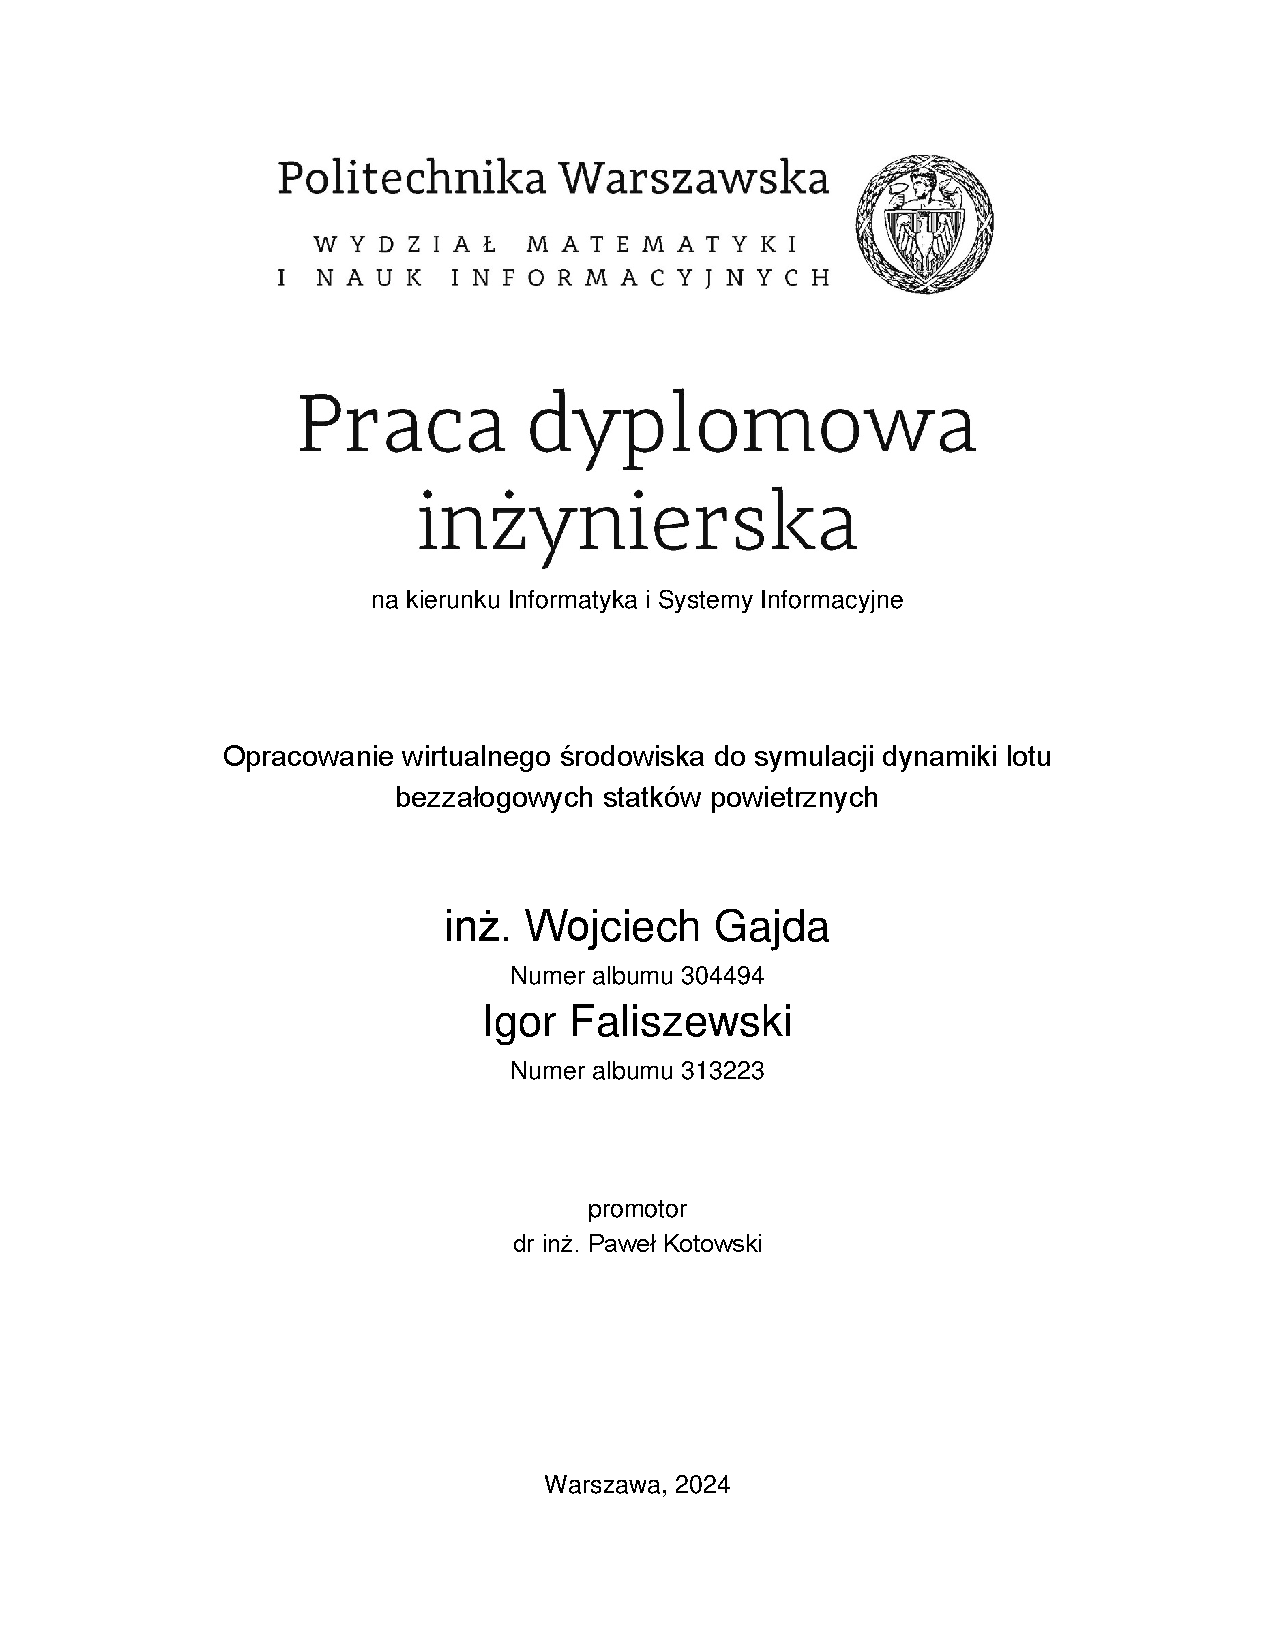
\includepdf[pages=-]{first_page.pdf}


\section*{Streszczenie}
Niniejsza specyfikacja stanowi opis systemu przeznaczonego do symulacji dynamiki lotu bezzałogowych statków powietrznych. System pozwala na prowadzenie symulacji lotu w czasie rzeczywistem, który dodatkowo jest prezentowany jest w postaci trójwymiarowej wizualizacji. W trakcie wykonywania lotu logowane są dane i mogą zostać wykorzystane do analizy lotu. Opracowany został uniwersalny model dynamiki pozwalający na swobodną konfigurację parametrów statku. Obejmuje on modyfikację właściwości mechanicznych, aerodynamicznych oraz konfigurację zespołów napędowych i~wpływu czynników zewnętrznych. Symulacja dynamiki rozszerzona została o system sterowania. System został zaprojektowany w sposobu ułatwiający zmianę parametrów statków i symulacji, tworzenie nowych konfiguracji statków oraz tworzenie i strojenie systemów sterowania. Przykładowych modelami, które mogą zostać zasymulowane są: stałopłatowiec, wielowirnikowiec i rakiety. 

\section*{Słowa kluczowe}

symulacja, grafika komputerowa 3D, bezzałogowy statek powietrzny, model dynamiki ruchu

%\newpage

%\section*{Abstract}

%\section*{Keywords}

%\newpage
%\tableofcontents

\newpage

\section{Słownik pojęć}

\textbf{Statek powietrzny} -- urządzenie zdolne do unoszenia się (lotu) w atmosferze. Statek powietrzny jest zdolny w sposób aktywny wpływać na kierunek i prędkość lotu. W przeciwieństwie do formalnej definicji termin obejmuje również konstrukcję niewykorzystujące oddziaływania powietrza w locie (rakiety).\\

\textbf{Bezzałogowy statek powietrzny, BSP} -- statek powietrzny, który nie wymaga do lotu załogi obecnej na pokładzie oraz nie ma możliwości zabierania pasażerów, pilotowany zdalnie lub wykonujący lot autonomicznie.\\ 

\textbf{Pocisk} -- obiekt wystrzelony lub upuszczony ze statku powietrznego, nieposiadający własnego napędu. Porusza się na wskutek oddziaływania pola grawitacji i wpływu powietrza. Nie posiada wyróżnionej orientacji.\\

\textbf{Ładunek} -- pocisk, na ogół upuszczany, który pozostaje związany z statkiem powietrzanym na sprężysto-tłumiącej linie. \\

\textbf{Stan obiektu} -- Opis położenia, orientacji i prędkości obiektu (pocisku lub statku powietrznego). Stan może zostać rozszerzony o dodatkowe informacje, takie jak: prędkości obrotowe poszczególnych silników, położenie powierzchni sterowych itd. \\

\textbf{Silnik fizyczny, silnik dynamiki} -- program komputerowy, którego zadaniem jest obliczenie położenia, orientacji i prędkości (kinematyki) statków powietrznych w zależności od sił działających na obiekt (dynamiki). \\

\textbf{Regulator} -- układ odpowiedzialny za generowanie rozkazów sterujących w oparciu o aktualny i zadany stan obiektu.\\

\textbf{Silnik graficzny} -- program komputerowy, którego zadaniem jest wizualizacja stanu obiektów i otoczenia.\\

\textbf{Agregator} --  program komputerowy, którego zadaniem jest zarządzaniem stanem aplikacji, obsługa przyłączających się aplikacji klienckich i zarządzanie procesami.\\

\textbf{Zasoby wizualizacji, assety} -- Modele i grafiki niezbędne do pracy aplikacji klienckiej.\\


\newpage

\section{Wstęp}

\subsection{O projekcie}

Symulacje komputerowe dynamiki ruchu stanowią użyteczne narzędzie w pracach inżynierskich. Pozwalają na analizę poprawności działania układu mechanicznego przed jego wyprodukowaniem. W szczególności w zagadnieniu jakim jest projektowanie bezzałogowych statków powietrznych, zastosowanie symulacji pozwala zminimalizować koszty wytworzenia poprawnie działającego systemu.

\subsection{Przegląd istniejących rozwiązań}

Historia symulatorów lotu sięga lat 30. XX wieku. Pierwotnie zastosowanie symulatorów sprowadzało się do szkolenia pilotów cywilnych i wojskowych. W znanej obecnie formie kompletne symulatory lotu stanowią rozbudowane systemy integrujące wysokiej klasy oprogramowanie z peryferiami mającymi wierne odwzorowanie kokpitu kierowanej maszyny. Symulatory wykorzystywane do treningu pilotów podlegają rygorystycznym regulacją prawnym i na ogół ich zadaniem jest odwzorowanie jednej konkretnej maszyny. Równolegle uproszczone wersje symulatorów zaczęły zyskiwać popularność w zastosowaniu cywilnym, jako element rozrywki. W szczególności gry komputerowe związane z lotem bardzo często poświęcały zgodność z rzeczywistością na rzecz lepszych odczuć użytkownika.\\

Na rynku dostępnych jest wiele środowisk symulacyjnych o różnym stopniu szczegółowości. Pełne systemy lotu stanowią produkt komercyjny projektowany na indywidualne zamówienie. Do najpopularniejszych dostępnych systemów sprzedawanych jako zamknięte oprogramowanie należą m. in.:

\begin{itemize}
\item Microsoft Flight Simulator -  seria komputerowych symulatorów lotu pozwalająca na symulację pilotowania różnych statków powietrznych. Założeniem jest wierne odtworzenie zachowania statków powietrznych, warunków pogodowych, jak również samych maszyn,
\item VBS (Arma) - środowisko symulacyjne do wizualizacji pola walki,
\item Warthunder - darmowa gra komputerowa wprowadzająca znaczną ilość historycznych i współczesnych modeli samolotów, których parametry zostały oparte na dostępnych i odtajnionych danych,
\item RealFlight - modelarski symulator lotu.
\end{itemize}

Istnieją również rozwiązania typu open-source, realizujące jedynie poszczególne zadania:

\begin{itemize}
\item JSBsim - rozbudowany silnik dynamiki lotu działający w czasie rzeczywistym,
\item Ardupilot, INAV, Betaflight - kompletne systemy sterowania dla modeli zdalnie sterowanych.
\end{itemize}


\section{Specyfikacja}


\subsection{Cel projektu}

Celem niniejszej projektu jest opracowanie wirtualnego środowiska do symulacji dynamiki lotu bezzałogowych statków powietrznych. System implementuje rozbudowany model dynamiki statków powietrznych wyposażonych w silniki rotorowe, silniki odrzutowe, powierzchnie nośne i powierzchnie sterowe. Pozwala na przeprowadzenie lotu symulowanym obiektem, którego parametry określane są przez konfigurację podaną przez użytkownika. Oprócz lotu system udostępnia dodatkowe funkcjonalności, takie jak możliwość strzału, upuszczenia ładunku, lotu z ładunkiem, rozpoznawania kolizji z otoczeniem.\\

Oprogromowanie ma stanowić zaawansowane narzędzie inżynierskie. Docelowym odbiorcą mają być zespoły R\&D opracowujące nowe konstrukcje latające lub prowadzące prace nad nowatorskimi systemami sterowania. System umożliwia zamodelowanie rzeczywistego modelu latającego i symulację jego lotu przed rzeczywistymi lotami próbnymi, co w rezultacie pozwoli na zminimalizowanie kosztów prototypowania. System rejestruje wiele parameterów lotu umożliwiając późniejszą analizę. Potencjalnymi odbiorcami systemu są uczelnie i instytuty naukowe, a także przedsiembiorstwa prowadzące prace badawczo-rozwojowe. Ze wzgledu na różnorodność zagadnień badanych przez wspomniane zespoły, trudno przygotować oprogramowanie uniwersalne. Z tego powodu system zostanie udostępniony na otwartej licencji MIT, aby umożliwić zespołom dostosowanie go do własnych potrzeb. Dla uławienie dalszego rozwoju projektu duży nacisk położony zostanie na przejrzystą implementację i realizację wzorców możliwych do ponownego użycia.\\

Otwarta licencja umożliwa również wykorzystanie systemu do celów rekreacyjnych i hobbistycznych. Szczególnym przypadkiem są modelarze, posiadający nierzadko znaczną wiedzę domenową i budujący swoje modele ze znaczną dbałością o szczegóły. Projektowany system może stanowić dla nich zamiennik profesjalnego oprogramowania, które ze względu na koszty licencji pozostawało dla nich niedostępne. Specyfika oprogramowania pozwala na użytkowanie go również w roli gry komputerowej. Oprócz wartości rozrywkowej, korzystanie z symulatora pozwala rozwijąc umiejętności pilotarzu, co przenosi się na rzeczywiste modele. Planowane jest wprowadzenie kilku funkcjonalności, których rolą jest jedynie poleszenie odczuć użytkonika aplikacji i zwiększenie przyjemności z korzystania z systemu.

\newpage

\section{Wstęp teoretyczny}


\subsection{Dynamika lotu}

Dynamika lotu jest dziedziną nauki skupiającą się na badaniu ruchu obiektów w atmosferze, zwłaszcza statków powietrznych. W założeniu bazuje ona na mechanice klasycznej. Jej znajomość pozwala na opracowanie modelu fenomenologicznego. \\

W trakcie prezentacji wprowadzone zostaną podstawowe pojęcia z zakresu modelowania obiektów dynamicznych oraz przedstawiony zostanie wykorzystany model dynamiki lotu symulowanych statków wraz ze szczegółowym omówieniem jego składowych. Ponadto omówione zostaną szczególne akcje które mogą wystąpić w trakcie symulacji takie jak kolizje z otoczeniem oraz odrzut po wystrzale.

\subsection{Sterowanie statkiem powietrznym}

Sterowanie statkiem powietrznym stanowi oddzielną dziedzinę zajmującą się analizą, w jaki sposób powinniśmy oddziaływać na statek, aby zachowywał się on w oczekiwany sposób. W przypadku niektórych statków odpowiedni system sterowania jest wręcz niezbędny, aby lot był możliwy. Sterowanie statkiem powietrznym w sensie teoretycznym jest klasycznym przypadkiem sterowania w pętli sprzężenia zwrotnego. Systemy sterowania wspomagają sterowanie na różnych poziomach niezależności: jako stabilizatory, autopiloty lub generatory trajektorii. \\

W trakcie prezentacji wprowadzone zostaną podstawowe pojęcia z zakresu sterowania obiektami dynamicznymi oraz przedstawione zostaną przykładowe konstrukcje pozwalające na sterowanie lotem.

\subsection{Wybrane zagadnienia z grafiki komupterowej 3D}

Grafika komputerowa to dyscyplina zajmująca się cyfrową syntezą i manipulacją treści wizualnych. Niezastąpionym elementem grafiki komputerowej jest procesor graficzny (GPU), który został zaprojektowany w taki sposób aby umożliwić na przeprowadzanie wielu niezależnych obliczeń jednocześnie. Są różne metody komunikacji z GPU. Jedną z nich jest OpenGL, a więc Open Graphics Library, który jest wielką maszyną stanu, pozwalającą na skonfigurowanie kontekstu oraz bezpośrednie rysowanie na ekranie. Potok renderowania zaczyna się od zdefiniowania danych wierzchołków, po ich przetworzenie, utworzenie prymitywów, przycinanie do ekranu, rasteryzację, przetwarzanie fragmentów, pikseli i ostatecznie zapisanie wyniku do buforu klatki. Jako programiści wpływ mamy na proces przetwarzania wierzchołków oraz przetwarzania fragmentów, kolejno za pomocą shaderów wierzchołkowych i fragmentowych. Pozwalają one za pomocą dedykowanego języka GLSL (Graphics Library Shader Language) manipulować w prosty sposób na przykład pozycję wierzchołków i kolory fragmentów. Shadery możemy wykorzystywać również shader geomterii, który został wykorzystany do utworzenia nowych wierzchołków reprezentujących linę. Sama linia jest zbiorem punktów wzdłuż krzywej łańcuchowej, która jest dobrym przybliżeniem rzeczywistej zwisającej liny. Na podstawie tych punktów tworzone są za pomocą algebry liniowej walce, które tym punktom nadają bryłę.


\newpage
\section{Bibliografia}

%\printbibliography
\nocite{*}

\printbibliography[type=book,heading=subbibliography,title={Literatura}]
\printbibliography[type=article,heading=subbibliography,title={Artykuły}]
\printbibliography[type=online,heading=subbibliography,title={Źródła internetowe}]

\end{document}\grid


\begin{comment}

Symulacje komputerowe dynamiki ruchu  W szczególności w zagadnieniu jakim jest projektowanie systemów sterowania do bezzałogowych statków powietrznych, zastosowanie takich narzędzi pozwala zminimalizować koszty wytworzenia poprawnie działającego systemu i przyśpieszyć jego rozwój i testowanie.

Celem niniejszej pracy jest opracowanie wirtualnego środowiska do symulacji dynamiki lotu bezzałogowych statków powietrznych. System implementuje podstawowy model dynamiki statków powietrznych wyposażonych w silniki rotorowe, silniki odrzutowe, powierzchnie nośne i powierzchnie sterowe. Pozwala na przeprowadzenie lotu symulowanym obiektem ktorego parametery określane są przez konfiguracje. System dzieli sie na serwer i aplikacje kliencką. Róznorodność modułów pozwala na realizacje róznych scenariusz (strzał, upuszczenie ładunku, kolizje, wpływ warunków srodowiskowych etc.)


\section{Model dynamiki statku powietrznego}

\begin{equation}
\begin{cases}
\dot{Y} =  T(Y) \cdot X + stabilizacja\\ 
A \cdot \dot{X} + \Omega (X) \cdot A \cdot X = F_g + F_a + F_d + F_o
\end{cases}
\end{equation}

gdzie:
\begin{itemize}
\item $Y$ - wektor pozycji i orientacji wyrażony w układzie globalnym
\item $X$ - wektor prędkości postępowej i kątowej w układzie związanym ze statkiem powietrznym
\item $A$ - macierz masowa
\item $\Omega$ - macierz gyroskopowa
\item $F_g$ - siła i moment pochodząca od siły grawitacji wyrażone w układzie związanym ze statkiem powietrznym
\item $F_a$ - siła i moment aerodynamiczny wyrażone w układzie związanym ze statkiem powietrznym
\item $F_d$ - siła i moment zespołów napędowych wyrażone w układzie związanym ze statkiem powietrznym
\item $F_o$ - siła i moment oddziaływań zewnętrznych napędowych wyrażone w układzie związanym ze statkiem powietrznym
\end{itemize}

\begin{equation}
Y = \begin{bmatrix}
x_{NED}\\
y_{NED}\\
z_{NED}\\
q_0\\
q_x\\
q_y\\
q_z
\end{bmatrix}
\end{equation}

\begin{equation}
X = \begin{bmatrix}
\dot{x}_b\\
\dot{y}_b\\
\dot{z}_b\\
P_b\\
Q_b\\
R_b
\end{bmatrix}
\end{equation}

\begin{equation}
F_g = R_{nb}(Y) \cdot  \begin{bmatrix}
0\\
0\\
g
\end{bmatrix}
\end{equation}

\begin{equation}
F_a = \frac{1}{2}\rho \cdot V_{tot}^2 S R_{wb} C_F \\
M_a = \frac{1}{2}\rho \cdot V_{tot}^2 S d R_{wb} C_F
\end{equation}

\end{comment}
